\section{Time Of Flight}

%  TOF
AMS-02 has four planes of TOF counters, plane 1 and 2 are above the magnet (Upper TOF), and plane 3 and 4 are below the magnet (Lower TOF) \cite{AMSTOFPaper1, AMSTOFPaper2}. Planes 1, 2, and 4 consist of eight plastic scintillator paddles, while plane 3 has ten paddles. The paddles have different lengths between 117 and 134 cm and a thickness of 1 cm. In the upper and lower TOF, the two planes are arranged in the X and Y directions as shown in figure \ref{TOFArrangement}. To avoid possible gaps between the paddles, the paddles are placed with a 0.5 cm overlapping. Each paddle is also equipped with 2 or 3 Photo-Multiplier Tubes (PMTs) on each end, which collect the light signal from the plastic scintillator and provide efficient particle detection.  \par
 
\begin{figure}[h]
\centering
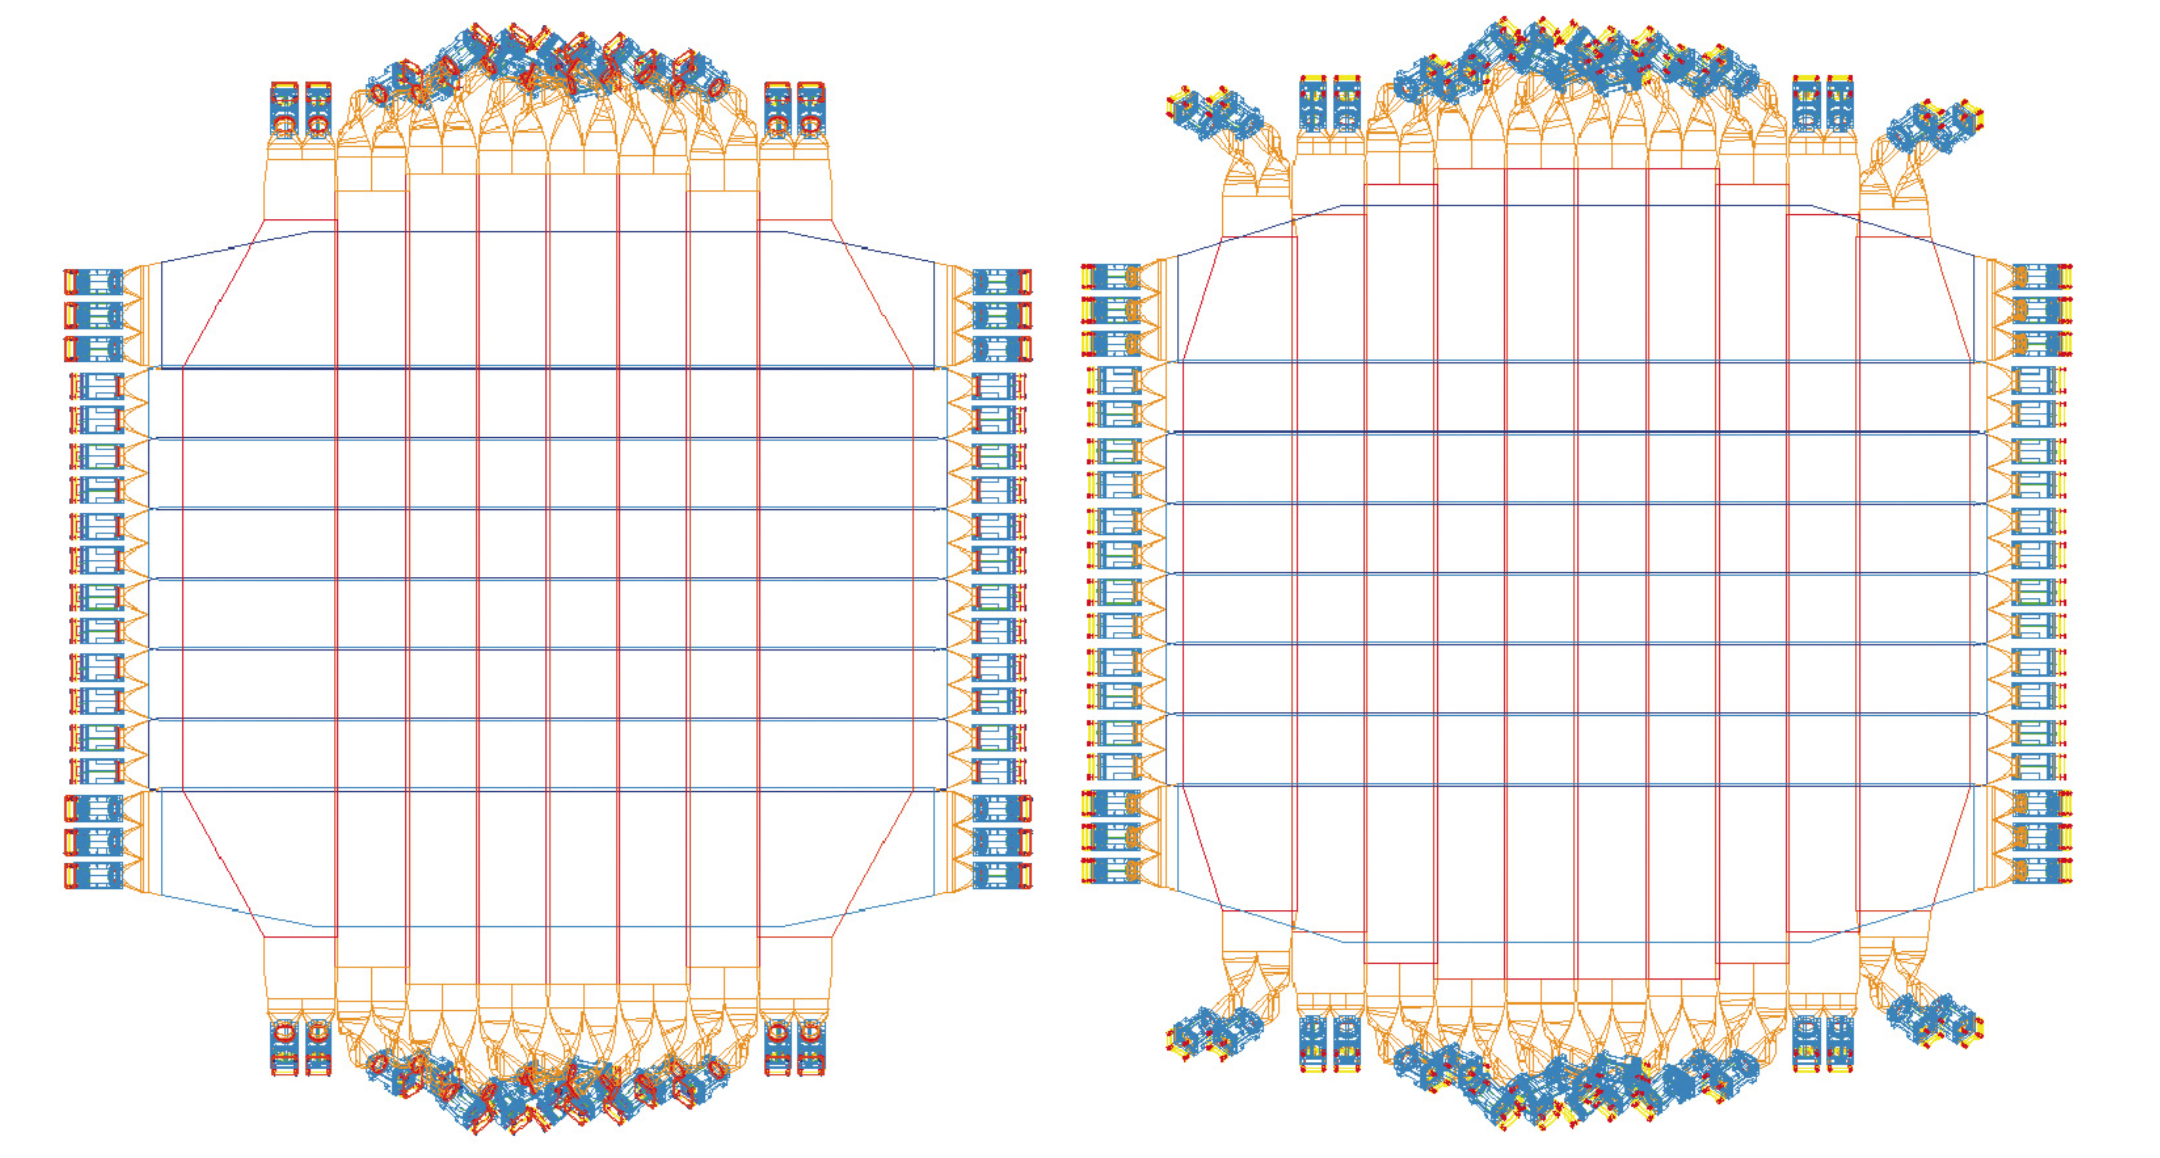
\includegraphics[width=0.8\textwidth, height=0.36\textheight ]{Figures/chapter3/TOF/Arrangement.png}
\caption[The TOF planes arrangement in the AMS-02 experiment.]{The TOF planes arrangement in the AMS-02 experiment. Left: Upper TOF and Right: Lower TOF \cite{TOFdetector}. }
\label{TOFArrangement}
\end{figure}

% TOF trigger
%Combining the information from all four planes, the TOF system can provide the particle trigger for the AMS-02 experiment. 
%More details on the trigger will be discussed in Section \ref{TriggerEfficiencySection}.  \par  

 % Time Resolution
The TOF system provides the particle's velocity by measuring the time difference between signals from the upper and lower TOF. Each counter's time resolution is around 160 ps, and the combined $\beta$ resolution is around $4 \%$ for $\beta \approx 1$ and $Z=1$ particles (figure \ref{TOFBetaResolution}). This provides the ability to discriminate between the up-going and down-going particles. Also, since the particle's mass is determined by: 

\begin{equation}
m=\frac{ZR}{\beta \gamma}
\label{MassEquation}
\end{equation}

combined with the rigidity measurement from tracker, the particle's mass can be obtained. \par  

%  Charge Resolution
Apart from measuring the velocity, the TOF can also provide the particle's charge. By measuring the ionization energy loss ${\rm{d}}E/{\rm{d}}X$, the charge of the particles can be independently obtained from the anode and dynode signals of the PMTs. The charge resolution is $\Delta Z=0.05$ for charge one particles (figure \ref{TOFChargeResolution}).  \par

\begin{figure}[H] 
\centering   
\subfigure[] { \label{TOFBetaResolution}    
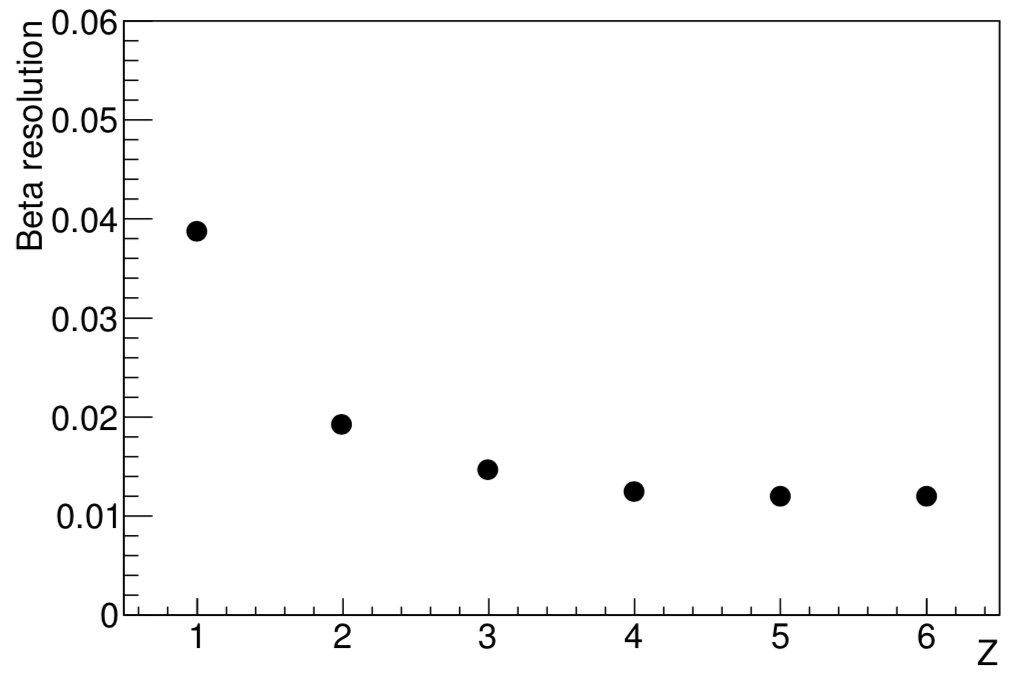
\includegraphics[width=0.45\columnwidth, height=0.225\textheight]{Figures/chapter3/TOF/TOFBetaResolution.png} 
}    
\subfigure[] { \label{TOFChargeResolution}    
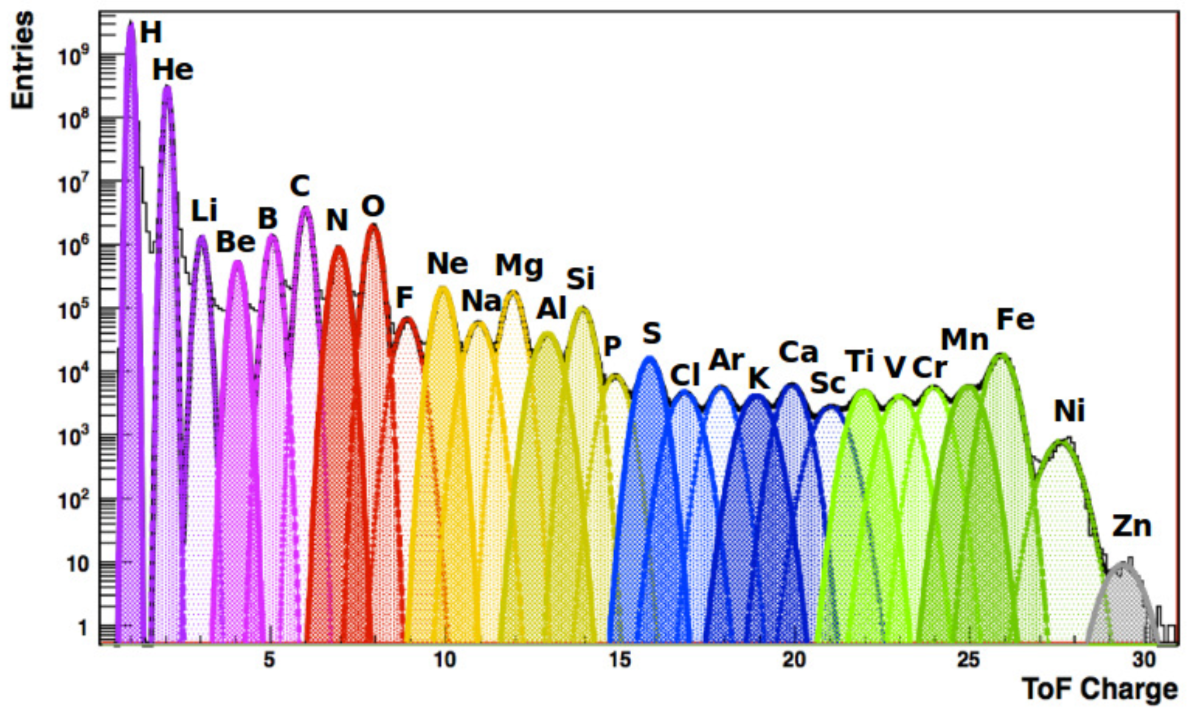
\includegraphics[width=0.45\columnwidth, height=0.225\textheight]{Figures/chapter3/TOF/TOFChargeResolution.png}    
}     
\caption[The TOF $\beta$ resolution and charge distribution.]{a) The TOF $\beta$ resolution as a function for particle charge \cite{TOFdetector}; b) The TOF charge distribution from protons (Z=1) up to Zinc (Z=30) \cite{TOFdetector}. }
\label{TOFReesolutions}    
\end{figure}

